\noindent Dans le cadre du projet pour \acrshort{pjcci}, une plateforme technologique sera mise à la disposition des gestionnaires du pont afin de les aider à prendre les décisions les plus responsables et raisonnables possibles. Mais la mise en service d'une solution innovante et fiable, qui concilie des algorithmes d'apprentissage profond, du temps réel, des nano-ordinateurs, et des conditions climatiques variables, est complexe. Dans une certaine mesure, l'essai va contribuer à la recherche de solutions afin de répondre au défi pour le domaine du transport actif et durable d'être soutenu par des solutions technologiques fiables (opérationnelles), l'objectif étant de pouvoir offrir des services de qualité et sécuritaires sur l'ensemble des quatre saisons.
\begin{comment}
\vspace{0.5\baselineskip}
\\
\noindent Il est difficile de trouver des jeux de données pour entrainer les réseaux de neurones pleinement connectés (\acrshort{fcn}) adaptés à la problématique. La technique de transfert d'apprentissage permet de démarrer d'une architecture qui a déjà appris avec un jeu d'images important (milliers d'images), et de lui faire apprendre davantage, en lui fournissant un plus petit jeu d'images (centaines d'images) de la nouvelle zone d'étude. Par exemple une architecture peut avoir appris à classifier des images de la Californie, aux États-Unis. Pour lui permettre de classifier des images de la Ville de Sherbrooke, il est souhaitable de lui fournir un nouveau jeu de données spécifique à cette ville afin qu'il s'adapte (ses paramètres) à cette région. Dans le contexte de cet essai, cela se traduit par réentrainer différents modèles avec des images de la piste multifonctionnelle du pont Jacques-Cartier.
\end{comment}
\vspace{0.5\baselineskip}
\\
\noindent La paramétrisation (des "hyper-paramètres") des réseaux de neurones est subtile et intuitive, et requière de l'expérience. C'est un processus d'essais-erreurs qui est couteux en temps, et risqué puisqu'il n'y a aucune garantie de succès. La technique d'apprentissage par transfert ("Transfer Learning" en anglais) permet d'hériter d'une architecture qui est déjà entrainée et paramétrée, et de l'adapter à d'autres problématiques, en lui fournissant un plus petit jeu d'images (une centaine) de la nouvelle zone d'étude. Cette technique permet un gain en temps puisque la phase de conception (analyse, architecture, configuration) est raccourcie de façon importante.
\begin{comment}
Par exemple l'architecture "VGG" prend 2-3 semaines d'entrainement \parencite{simonyan_very_2015} avec 4 \acrshort{gpu} Titan Black (NVIDIA), coutant 1 200 \$US (Amazon.com) chacun (pour un total de 4 800\$US, et cela juste pour les \acrshort{gpu}s, qui ne sont qu'un des éléments de l'infrastructure nécessaire). Étant donné que de multiples tentatives sont nécessaires (cycles essai-erreur), la stratégie est d'entrainer plusieurs modèles en parallèle afin d'accélérer le développement, ce qui implique un cout élevé en infrastructure.
\end{comment}
La problématique pour l'essai est de trouver l'architecture qui est la plus adaptée pour répondre au besoin, et il en existe des milliers \parencite{koh_model_2018}. La recherche dans la littérature permet heureusement de limiter les choix et donner des pistes \parencite{zheng_real-time_2020, nguyen_mavnet_2019, nvidia_jetson_2019-1}. 
\vspace{0.5\baselineskip}
\\
\noindent Même si les scores sont satisfaisants lors de la phase de test du modèle, la réalité du terrain peut surprendre. Les tests d'acceptation du modèle doivent se faire en dehors de l'environnement d'entrainement (laboratoire), dans les conditions réelles (luminosité, angle, hauteur, etc.) sur le terrain d'implémentation. Dans le jargon de l'intelligence artificielle et des réseaux de neurones, c'est l'inférence\footnote{Le terme "inférence" est utilisé lorsqu'un modèle, entrainé avec un échantillon de la population, est appliqué pour pouvoir donner une conclusion pour d'autres échantillons de la population (déduire un chien ou un chat sur une image). Le terme "prédiction" est utilisé lorsqu'un modèle, entrainé avec un échantillon de la population, est appliqué pour déduire une valeur selon une ou plusieurs variables (la température selon la localisation et l'altitude).} \parencite{copel_whats_2016, nvidia_jetson_2019-1}. De plus, le système hôte, dans notre cas le nano-ordinateur NVIDIA Jetson Nano, est conçu avec une architecture matérielle limitée (\acrshort{gpu}, \acrshort{cpu}s, mémoire, taux de transfert, alimentation). 
\vspace{0.5\baselineskip}
\\
\noindent La segmentation sémantique (figure \ref{fig:semantic_segmentation_vs_others}) est une forme de classification d'image, pixel par pixel, qui tire profit des dernières évolutions de la classification supervisée grâce aux réseaux de neurones pleinement connectés (\acrshort{fcn}), et qui peut être réalisée en temps réel avec des nano-ordinateurs \parencite{long_fully_2015, blanco-filgueira_deep_2019}. Les images doivent être de haute résolution, ce qui nécessite d'avoir à disposition un système informatique capable de fournir une puissance de calcul appropriée, particulièrement pour la manipulation de la mémoire et des nombres flottants pendant l'inférence \parencite{mody_low_2018}. Leur application par des nano-ordinateurs est un défi en raison de la faible consommation d'énergie (Watts) et de la puissance de calcul limité de ces derniers \parencite{copel_whats_2016}.
\begin{figure}[H]
    \centering
    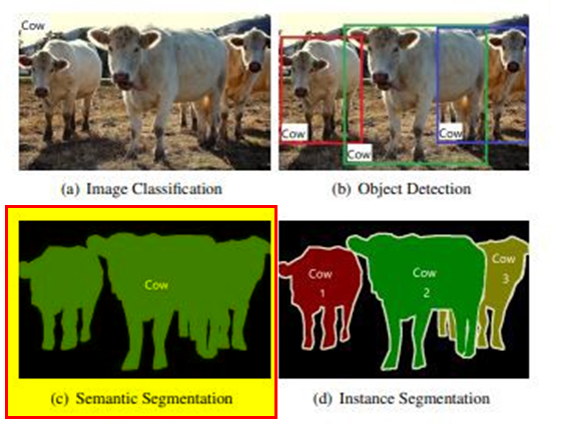
\includegraphics[width=0.75\textwidth]{semantic_segmentation_vs_others}
    \caption[Segmentation semantic]{Segmentation semantic\parencite[p.~1]{wu_recent_2019}}
    \label{fig:semantic_segmentation_vs_others}
 \end{figure}
\noindent Il existe différents cadres applicatifs pour l'entrainement de modèles \acrshort{ia}, tels que PyTorch ou TensorFlow. L'inconvénient est d'avoir à installer pour chacun leur propre environnement de développement et d'inférence, ce qui augmente les efforts et les coûts. Le cadre applicatif ONNX a été conçu pour pallier cette contrainte. En effet, il uniformise les architectures des modèles, et simplifie la mise en service grâce à l'installation d'un unique cadre applicatif. NVIDIA fournit avec le Jetson Nano une plateforme applicative qui supporte les modèles convertis au format ONNX, et offre donc une solution supportant l'interopérationabilité des modèles \acrshort{ia}. 